\chapter{Measures and dimensions}
\label{chap:intro}



Felix Hausdorff introduced what is now known as the Hausdorff dimension in 1918 \cite{hausdorff} as a means of studying geometric objects for which the classical notions of dimension and size fail. The sets studied in this context are often irregular such as trajectories of Brownian motion, the Cantor set and the Mandelbrot set, see Figures \ref{fig:examples1} and \ref{fig:examples2} for a few examples. Whilst there is no formal definition behind the term `irregular objects', one should think of them as possessing infinitesimal detail, that is, as one zooms in on a certain part of the object, new, interesting behaviours exhibits. Mandelbrot \cite{mandelbrot} coined the term \textit{fractal} in 1977 to encompass the wide range of examples satisfying this concept and since then there has been an increasing interest in the study of fractals, both theoretical and applied. As many naturally occurring objects are messy and chaotic, fractals are suitable models for their study, seeing use in a wide range of disciplines such as finance and the life sciences, as in \cite{diieva, diieva2}. The applications in theoretical mathematics are also numerous, having profound influences on number theory and dynamical systems among others. 


\begin{figure}
\begin{subfigure}{.5\textwidth}
  \centering
  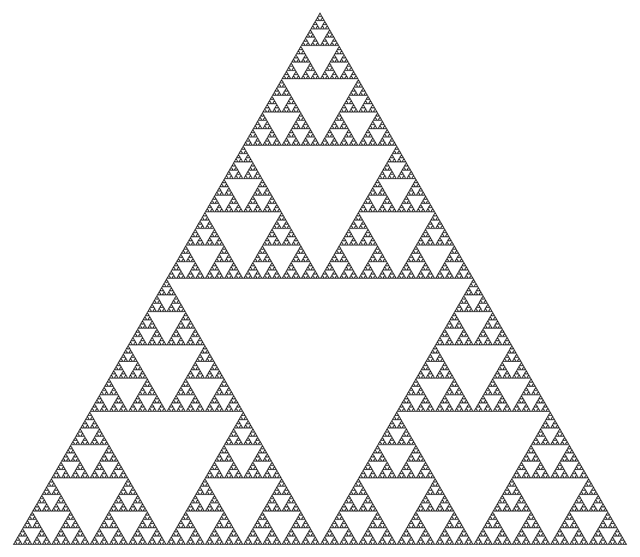
\includegraphics[width=.8\linewidth]{pics/intro/sierpinski.png}
  \label{fig:sfig1}
\end{subfigure}%
\begin{subfigure}{.5\textwidth}
  \centering
  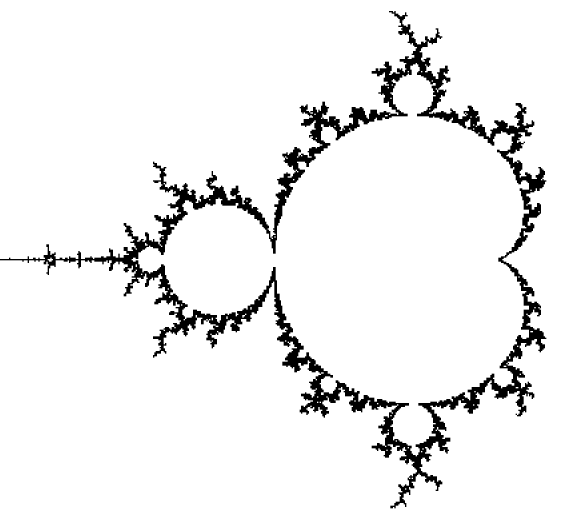
\includegraphics[width=.8\linewidth]{pics/intro/Boundary_mandelbrot_set.png}
  \label{fig:sfig2}
\end{subfigure}
\caption{A few well studied fractal sets. The first one is a Sierpi\'nski triangle and the right one is the boundary of the Mandelbrot set}
\label{fig:examples1}
\end{figure}



Since the introduction of the Hausdorff dimension, many other notions of dimension have been defined, each with its own unique properties. The underlying principle of all definitions of dimension is that they should quantify how much of a set is within a given space asymptotically; how they quantify this and which space they restrict to is what distinguishes them. We will mostly be interested in the \textit{Assouad} and \textit{lower dimensions} in this thesis, but one of the interesting aspects of fractal geometry is the interaction between the different notions of dimension and so other dimensions will arise throughout to place this work into the greater context. The Assouad dimension, when thinking about the governing idea of a dimension, is interested in understanding how much space a given set takes up with respect to a small scale $r$ when restricted to a ball of size $R$, where $R$ is close to zero but still greater than $r$. In particular it focuses on the balls in which the studied set takes up as much space as possible. This means the Assouad dimension provides an \textit{extremal} notion of size of an object, often being the largest of the main dimensions and discards information about the rest of the set. This is complemented by the lower dimension which provides similar details but focusing on where the set is the least space filling.  



\begin{figure}[h]
\begin{subfigure}{.5\textwidth}
  \centering
  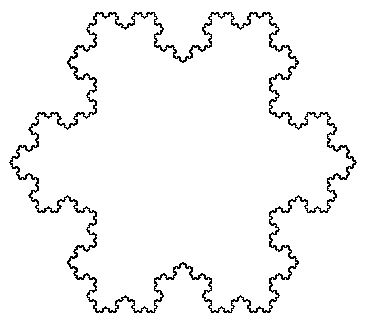
\includegraphics[width=.8\linewidth]{pics/intro/vonKoch.png}
  \label{fig:sfig1}
\end{subfigure}%
\begin{subfigure}{.5\textwidth}
  \centering
  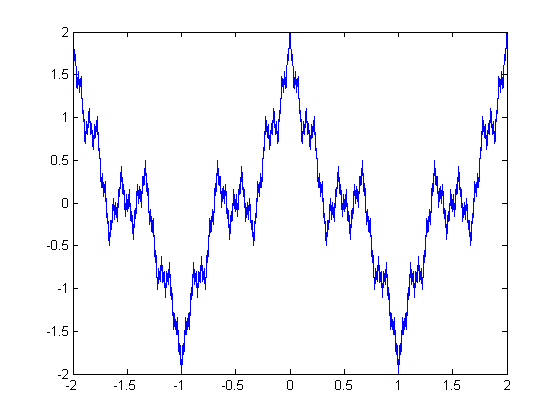
\includegraphics[width=.8\linewidth]{pics/intro/weierstrass.png}
  \label{fig:sfig2}
\end{subfigure}
\caption{More examples of fractals. Left is a von Koch snowflake and right the graph of the Weierstrass function}
\label{fig:examples2}
\end{figure}



During the study of these irregular geometric objects, a desire to study the regularity of measures supported on them has arisen, leading to the notion of dimension of a measure. Naturally there are several definitions of dimension of a measure, each one often being related to a dimension of sets. The study of these dimensions of measures has recently contributed to significant advances in our understanding of sets that were previously considered almost too complex to work with, as in \cite{hochman}. If a geometric dimension tells us roughly how much of a set is within a given area, a dimension of measures is interested in how thea measure is distributed over such objects. The Assouad and lower dimensions have corresponding dimensions of measures which, in this thesis, will be called the \textit{upper} and \textit{lower regularity dimensions} respectively. Whilst the Assouad and lower dimensions have seen an increasing popularity in the recent years, the regularity dimensions are only starting to attract attention and much of this thesis will be interested in expanding on their basic properties and their interactions with other dimensions. Like the Assouad dimension, the regularity dimensions are also extremal notions of size, a fact exemplified by noting the upper regularity dimension of non-doubling measures is always infinity. The links between doubling measures, a standard regularity property in the literature, and the upper regularity dimension will be expanded upon. 





\section{Dimensions of sets}
\label{sec:intro-sets}
\nomenclature[X]{$(X,d)$}{metric space with associated distance function}

In this section we will introduce and define several different notions of dimension that will occur throughout this thesis. Dimensions are concerned with the size of objects and so one must first establish a notion of distance. This is done by studying subsets of metric spaces $(X,d)$; for clarity we will often refer to the space $X$ with the metric being implicitly defined. One should assume $X$ is compact, however this is not always needed and in fact there are some particularly beautiful results that will be referenced in Section \ref{sec:intro-ass} that hold for non-compact sets which are helpful when studying number theoretic questions. When discussing the distance between points we will use the notation $d(x,y)$ to be the distance between the points $x,y \in X$ where the space is clear. If multiple metric spaces are being considered simultaneously the notation $d_X(x,y)$ will be adopted to specify the metric space $X$ in which the distance is taken. We will later study measures on metric spaces and we take the associated $\sigma$-algebra to be the Borel $\sigma$-algebra given the underlying metric. We will not constantly specify the $\sigma$-algebra for notational convenience.

Whilst we aim to be precise here, this will still be a brief introduction and the interested reader should see the standard books \cite{falconer, falconer2, mattila} for an extensive introduction to many of these topics. 



\subsection{Hausdorff and box dimensions}
\label{sec:intro-haus-box}

The Hausdorff dimension is arguably the most commonly studied notion of dimension in the fractal geometry literature and has been since its inception in 1918 by Hausdorff. Whilst its construction is somewhat technical, involving the Hausdorff measure, the advantages are significant, endowing this dimension with many interesting properties. 

\nomenclature[.]{$\lvert \cdot \rvert$}{diameter of a set}
Let $F\subseteq X$, $s\ge 0$ and $r > 0$. We first define a $r$-cover of $F$ as a cover of $F$ by open sets of diameter at most $r$. We will use $\lvert \cdot \rvert$ to denote the diameter of a set, so $\lvert F \rvert = \sup \left\{d(x,y) \colon x,y \in F \right\}$ for any $F\subseteq X$ . Then the $r$-approximate $s$-dimensional Hausdorff measure of $F$ is defined by 
\[
\mathcal{H}^s_r (F) = \inf\left\{ \sum_{i\in I} \lvert U_i \rvert^s \colon \left\{U_i \right\}_{i\in I} \text{ is a $r$-cover of }F  \right\}.
\]
Taking the limit as $r \rightarrow 0 $ gives the $s$-dimensional Hausdorff (outer) measure $\mathcal{H}^s(F) = \lim_{r\rightarrow 0} \mathcal{H}^s_r(F)$. This finally leads to the \textit{Hausdorff dimension} of $F$ given by
\[
\dim_\H F = \sup\left\{s \ge 0 \colon \mathcal{H}^s(F) = \infty\right\} = \inf\left\{s\ge 0 \colon \mathcal{H}^s(F) = 0\right\}.
\]
\nomenclature[dimH]{$\dim_\H$}{Hausdorff dimension}
As mentioned before, calculating this dimension from first principles is usually quite difficult, but due to the definition following from the Hausdorff measure it is well behaved. In particular, it is countably stable. We will later be interested in calculating the Hausdorff dimension of a few different sets, notably self-similar with the Strong Separation Condition (SSC), Bedford-McMullen carpets and sequences of numbers decaying to zero such as $\left\{1/n \colon n\in \mathbb{N}\right\}\cup \left\{ 0\right\}$. For the first two, formula already exist which will be stated when needed and for the last one, as it is a countable set, it is easily seen to have zero Hausdorff dimension due to the countable stability of the dimension.

A coarser but easier to compute dimension was desired, without straying too far from the Hausdorff dimension. This lead to the upper and lower box dimensions in the 1920s, as in \cite{bouligand}. Given $F\subseteq X$, take $N(F,r)$ to be the smallest number of sets needed in a $r$-cover of $F$. Then the \textit{upper} and \textit{lower box dimensions} are defined by
\nomenclature[N(F]{$N(F,r)$}{covering number of a set $F$ by sets of radius at most $r$}
\nomenclature[dimB]{$\dim_{\textup{B}}$}{box dimension}
\[
\ubox F = \limsup_{r \rightarrow 0} \frac{-\log N(F,r)}{\log r}   \quad \text{ and } \quad \lbox F = \liminf_{r \rightarrow 0} \frac{-\log N(F,r)}{\log r}. 
\]
 When $\ubox F = \lbox F$, we simply talk about the \textit{box dimension} of $F$ and denote it $\dim_{\textup{B}} F$. This will be the case in all the examples in this thesis for which the box dimension is studied. In reality we will take $N(F,r)$ to be the smallest number of balls of radius $r$ required to cover $F$, or the smallest number of squares of side lengths $r$. These changes will not modify the box dimensions of a set and will greatly simplify calculations. Of particular interest in real world applications, one can take $N(F,r)$ to be the number of squares in the $r$-mesh that intersect $F$ and a computer can then calculate this number for a sequence of scales, approximating the box dimension to a reasonable degree such as in \cite{diieva}.

A simple example of the box dimension's coarser behaviour is the set $F = \left\{1/n \colon n \in \mathbb{N} \right\} \cup \left\{ 0\right\}$ which has box dimension $1/2$ despite having zero Hausdorff dimension. The proof of this is not trivial so we include it here for completeness. 

Let $r>0$, we wish to study $N(F,r)$ for $r$ small. First note, that for any $k \in \mathbb{N}$, 
\[
\frac{1}{k} - \frac{1}{k+1} = \frac{1}{k(k+1)}.
\]
Thus the distances between points in this set behave like $1/k^2$. Choose $n \in \mathbb{N}$ to be the largest integer such that $1/n(n+1) > r$. We will then split the cover of $F$ into two parts, one half where the distances between points are smaller than our covering sets and the other where they are greater. In the second case it is clear that one ball is needed for each element for a full cover, so $n$ balls. When the distances between points are smaller than $r$ we will need an essentially maximal covering to cover all such elements as the set starts to behave like an interval with respect to the scale $r$. Therefore covering the first section is akin to covering the interval $[0,1/n]$. Hence
\[
N(F,r) \ge N([0,1/n]\cap F,r) \ge n/2 \ge r^{1/2}/4
\]
and
\[
N(F,r) \le N([0,1/n],r) + n \le \frac{3}{4} r^{-1/2}, 
\]
completing the proof that $\dim_{\textup{B}} F = 1/2$.


\subsection{Assouad and lower dimensions}
\label{sec:intro-ass}

The notion of dimension that will most interest us in this thesis is the Assouad dimension, named after Patrice Assouad who proved the Assouad embedding theorem in the 70s \cite{assouad1, assouad2} which relates the Assouad dimension of a metric space with nearly bi-Lipschitz embeddings into Euclidean space. The notion of the dimension itself can be traced back to a paper of Bouligand in 1928 \cite{bouligand} and then Larman in the 60s \cite{larman1,larman2}. The \textit{Assouad dimension} of $F \subseteq X$ is defined by 
\nomenclature[dimA]{$\Assouad$}{Assouad dimension}
\begin{multline*}
\dim_{\text{A}} F = \inf \Bigg\{ s \geq 0 \, \,  : \, \exists \text{ constant } C > 0 \text{ such that, for all } \, \, 0< r< R,\\ \text{ we have  }\sup_{x\in F} N_r (B(x,R)\cap F) \leq C\left(\frac{R}{r}\right)^{s} \Bigg\}.
\end{multline*}
Here and throughout, $B(x,R)$ denotes a closed ball in $X$ of centre $x$ and radius $R$.
\nomenclature[B(x]{$B(x,R)$}{ball of centre $x$ and radius $R$}

As the supremum is taken over all points in the set $F$, the dimension returns local information, specifying how the set behaves in its most dense regions. This contrasts with the global averages that the Hausdorff and box dimensions provide. Usually the Assouad dimension will be the largest of dimensions a space can take. This local `largeness' is important in embedding problems since if there is an embedding that holds for the most extreme subsets, then it will likely hold for the rest of the set. 

Whilst the name comes from an application to embedding theory, the Assouad dimension has seen much study in a number of different areas, including further embedding theory questions \cite{olson02, olson10, robinson}, quasi-conformal geometry \cite{heinonen, tyson, mackaytyson}, classic fractal geometry \cite{fraser-kaenmaki-proj, fraser-todd, tros, orponen, ldr} and even some applications to number theory \cite{FY, fraser-saito-yu}. This list is non-exhaustive and we recommend \cite{robinson, Fr} for further discussion of this dimension including many of its basic properties, however these do not cover the multitude of new results which have appeared in the past few years. 

A key notion that is highly related to the Assouad dimension is the concept of a doubling space. A space $X$ is doubling if there exists a constant $M > 0$ such that, for any $R > 0$ and any $x \in X$, one can cover the ball of radius $R$ and centre $x$ by at most $M$ balls of radius $R/2$. It is known that a space is doubling if and only if it has finite Assouad dimension, see \cite[Lemma 9.4]{robinson} for a proof. Thus, the Assouad dimension can be seen as quantifying how doubling a space is.

We are also interested in the following measure theoretic formulation of the Assouad dimension due to \cite{luksak, konyagin} for complete metric spaces: 
\begin{align*}
   \dim_{\text{A}} F = \inf \Bigg\{ s \geq 0 \, \,  : \, \exists \text{ a Borel probability measure } \mu \text{ fully supported by }F \\  
   \text{ and constant }C > 0\text{  such that, } \text{for all } \, \, 0< r< R, \\ 
   \text{ we have  }  \sup_{x\in F} \frac{\mu(B(x,R))}{\mu(B(x,r))} \leq C\left(\frac{R}{r}\right)^{s} \Bigg\}. 
\end{align*}
As the spaces $X$ are assumed to be compact, the completeness condition is always satisfied for the examples studied here. This definition allows us to relate the purely geometric concept of dimension with a measure theoretic study. This can be advantageous when more is known about the measures than the set itself, such as in \cite{fraser-howroyd1}. More importantly, this will lead to the notion of `Assouad dimension' of a measure, which will be further explored in the next section. 


As the Assouad dimension provides coarse, extremal information, it is natural to consider an analogous dimension which studies regions of the set which require very few balls to cover. This leads to the definition of the lower dimension, first studied by Larman \cite{larman1,larman2}. The \textit{lower dimension} of $F \subseteq X$ is 
\nomenclature[dimL]{$\lowerdim$}{lower dimension}
\begin{multline*}
\dim_{\text{L}} F = \sup \Bigg\{ s \geq 0 \, \,  : \, \exists \text{ constants }C, \rho > 0 \text{ such that, for all } \, \, 0< r< R \leq \rho,\\ \text{ we have  }\inf_{x\in F} N_r (B(x,R)\cap F) \geq C\left(\frac{R}{r}\right)^{s} \Bigg\}.
\end{multline*}
A careful reader would remark that this definition requires the radii $r< R$ to be bounded above by some constant, often taken to be the diameter of $F$. This is not needed in the Assouad dimension but here, without this condition, the lower dimension would always be zero. As the objects studied in this thesis are compact this requirement is easily satisfied. The lower dimension has seen less study, partially due to a few undesirable properties that it possesses, but when studying many of the main examples of fractals it behaves as expected and results for the Assouad dimension can often be transposed to the lower dimension. 

Like the Assouad dimension, the lower dimension also has a related regularity property. A space $X$ is uniformly perfect if there exists a constant $K > 1$ such that for any $x \in X$ and $R > 0$, there exists $y \in X \cap \left(B(x, R) \setminus B(x, R/K)\right)$. One can in fact show that a set is uniformly perfect if and only if it has positive lower dimension, see \cite[Lemma 2.1]{anti1} where the lower dimension is called the lower Assouad dimension. One of the main problems with the lower dimension is that the lower dimension of any set which contains an isolated point is always zero. Thus, restricting to uniformly perfect spaces would easily avoid this difficulty. 

Bylund and Gudayol \cite{bylund} proved the following result linking measures and lower dimension, similar to \cite{luksak, konyagin}
\begin{align*}
\dim_{\text{L}} F = \sup \Bigg\{ s \geq 0 \, \,  &: \, \exists \text{ a doubling Borel probability measure } \mu \text{ fully } \\  
&\text{supported on }F \text{ and constants }C, \rho > 0  \text{ such that, } \\ 
\text{for all } &\, \, 0< r< R \leq \rho, \text{ we have  }\inf_{x\in F} \frac{\mu(B(x,R))}{\mu(B(x,r))} \geq C\left(\frac{R}{r}\right)^{s} \Bigg\}.
\end{align*}
Compared to the measure theoretic definition of the Assouad dimension, this definition is essentially as expected, except for the restriction to doubling measures. A measure $\mu$ supported on $X$ is doubling if there exists a constant $C(2) > 1$ such that for all $x$ in the support of $\mu$ and $R > 0$ we have $\mu( B(x,R)) \le C(2) \mu(B(x,R/2))$; these measures will be discussed further in the next section. Restricting to doubling measures forces the measure to truly capture the entirety of the set, in the same way that focusing on fully supported measures is required to avoid part of the space being completely ignored and therefore losing vital information. However, this is not needed for the Assouad dimension as non-doubling measures will provide infinity as the upper bound to the dimension and so will not affect the Assouad dimension. 


For a general compact set $F$ the following relations were shown to hold by \cite{Fr, larman1, larman2}:
\[
\lowerdim F \le \dim_\H F \le \lbox F \le \ubox F \le \Assouad F.
\]
These inequalities can be, and often are, strict, with many interesting examples existing in the literature demonstrating the different combinations of equalities and inequalities possible. For example we have seen that the set $F=\left\{1/n \colon n \in \mathbb{N} \right\} \cup \left\{0 \right\}$ has zero Hausdorff dimension and box dimension equal to $1/2$. As the lower dimension is a lower bound to the Hausdorff dimension, $F$ will also have lower dimension zero and we will prove shortly that it has full Assouad dimension. On the other hand, for a self-similar set satisfying a suitable separation condition, all of these dimensions are equal. 

The proof that $F=\left\{1/n \colon n \in \mathbb{N} \right\} \cup \left\{0 \right\}$ has full Assouad dimension is quite similar to the proof of its box dimension, we show this to get a better feel for the Assouad dimension.

As we wish to prove the Assouad dimension is full, we simply need to find a lower bound, the upper following from the dimension of the ambient space. The most common way of doing this for the Assouad dimension is to find sequences of $x_n \in F$, and $0<r_n < R_n$ such that $R_n/r_n \rightarrow \infty$ and $N(F \cap B(x_n, R_n), r_n ) \ge CR_n/r_n$ for some constant $C>0$. The extremal behaviour of this set exhibits around 0 so we simply choose $x_n = 0$ for all $n$. To use the previous work on the box dimension, let $R_n = 1/n$ and $r_n = 1/n^2$. From before, $F\cap B(0,R_n)$ is the part of $F$ where the differences between points is less than $1/n^2$ so covering this subset is like covering $[0,1/n]$. Thus
\[
N(F \cap B(0, 1/n), 1/n^2 ) \ge n/2 = \frac{1}{2} \left( \frac{R_n}{r_n}\right)
\]
as desired.





\section{Dimensions of measures}
\label{sec:intro-measures}

\subsection{Upper regularity dimension}
\label{sec:intro-upper-reg}

As eluded to previously, the measure theoretic definitions of dimension lead to a natural notion of `Assouad dimension' of a measure which gives a quantifiable description of the extremal local scaling of the measure. This was first defined in \cite{anti1,anti2} under the name upper regularity dimension and studied in the context of inhomogeneous self-similar sets and Whitney covers. Let $\mu$ be a locally finite Borel measure on $X$ and write $\text{supp}(\mu) = \left\{ x \in X \colon \mu(B(x,r)) > 0 \textup{ for all } r > 0 \right\}$ for the support of $\mu$. In general, one should assume a measure is locally finite Borel unless otherwise stated. The \textit{upper regularity dimension} of $\mu$ is defined by 
\nomenclature[supp]{$\text{supp}$}{support of a measure}
\nomenclature[dimregu]{$\urdim$}{upper regularity dimension}
\nomenclature[mu]{$\mu$}{a measure}
\begin{align*} 
\urdim \mu = \inf \Bigg\{ s \geq 0 \, \,  : \,  \text{ there exists a  constant }C  > 0\text{  such that,} \\ \text{for all } 0< r< R  \text{  and all }x \in \text{supp} (\mu), \\ \text{we have }  \  \frac{\mu(B(x,R))}{\mu(B(x,r))} \leq C\left(\frac{R}{r}\right)^{s} \Bigg\},
\end{align*}
taking $\inf \emptyset = + \infty$. 

Combining this definition and the measure theoretic formulation of the Assouad dimension, the following can be deduced for a complete metric space $F$
\begin{equation}\label{equa:ass-reg-relation}
    \dim_{\text{A}} F = \inf \left\{ \overline{\dim}_{\text{reg}} \mu \,  \colon \, \mu \text{ is a measure fully supported on } F\right\}.
\end{equation}
This relationship has led to a number of people calling the upper regularity dimension the Assouad dimension, such as in \cite{hare-hare-tros, hare-troscheit, fraser-kaenmaki-proj}. As the papers this thesis is based upon use the terminology upper regularity dimension, we will continue to do the same; however, the term Assouad dimension is growing in popularity and will likely become the standard notation in the future.

As can be seen in equation \eqref{equa:ass-reg-relation}, the upper regularity dimension of a measure is always bounded below by the Assouad dimension of its support. In some cases the upper regularity dimension will even attain the Assouad dimension of the space, for example \cite[Theorem 2.3]{fraser-howroyd1}. However K\"aenm\"aki and Lehrb\"ack constructed a wide class of sets for which the Assoaud dimension of such a set $F$ is always strictly smaller than the upper regularity dimension of any doubling measure supported on $F$, see  \cite{anti2} and \cite{konyagin} for their inspiration. Much of this work will be dedicated to placing the upper regularity dimension in context with other notions of dimension, both generally and for specific examples.

A measure, like a space, can be doubling. Whilst the name doubling comes from the standard definition where measures of two balls are compared, with the radius of one ball being twice that of the other's, one can generalise this to any ratio between the radii. Formally, a measure $\mu$ is \textit{doubling} if and only if, for some $\theta > 1$, there exists a constant $C(\theta) > 1$ such that for all $x$ in the support of $\mu$ and $R > 0$ the following holds
\nomenclature[C(theta]{$C(\theta)$}{doubling constant with respect to the ratio $\theta$}
\[
\mu(B(x,R)) \le C(\theta) \mu(B(x,R/\theta)).
\]
Recalling a space is doubling if and only if it has finite Assouad dimension, it turns out that the upper regularity dimension behaves similarly. That is a measure is doubling if and only if the measure has finite upper regularity dimension. A proof of this can be found in \cite[Lemma 3.2]{kaenmakinew} and will be further explored in the Chapter 3. 


\subsection{Lower regularity dimension}
\label{sec:intro-lower-reg}


As the lower dimension is a natural dual of the Assouad dimension, so is there an analogue of the upper regularity dimension, called the lower regularity dimension. Inspired by \cite{bylund}, a measure $\mu$ on a metric space $X$ has \textit{lower regularity dimension} defined by 
\nomenclature[dimregul]{$\lrdim$}{lower regularity dimension}
\begin{align*} 
\underline{\dim}_{\text{reg}} \mu = \sup \Bigg\{ s \geq 0 \, \,  : \,  &\,\text{ there exists a  constant }C  > 0\text{  such that, for all }  \\ & \, 0< r< R < \lvert \text{supp}(\mu)    \rvert \text{  and all $x \in \text{supp} (\mu)$, we have }  \\  & \hspace{5cm} \frac{\mu(B(x,R))}{\mu(B(x,r))} \geq C\left(\frac{R}{r}\right)^{s} \Bigg\}.
\end{align*}
The lower regularity dimension quantifies the minimal local scaling of a measure and many of the ideas that have been discussed regarding the upper regularity dimension carry over to the lower analogue. As with the lower dimension, $R$ is bounded above by a constant in this definition; without such a constraint the lower regularity dimension would be always zero.

A definition of the lower dimension of a set $F\subseteq X$ can be deduced purely in terms of the dimension of measures
\begin{equation}
    \dim_{\text{L}} F = \sup \left\{ \lrdim \mu \,  \colon \, \mu \text{ a doubling probability measure fully supported on } F\right\}.
\end{equation}
This has lead to the lower regularity dimension being called the lower (Assouad) dimension in the literature, such as in \cite{hare-troscheit}. This also implies that the lower regularity dimension is an upper bound to the lower dimension, with examples for both equality and strict inequality of the two existing.

Being consistent with the previous section, one can state a definition for a measure to be \textit{uniformly perfect}; such measures were recently called reverse-doubling in \cite{anti2} due to the resemblance with doubling measures. A measure $\mu$ is uniformly perfect if for any $\theta > 1$ there exists a constant $K(\theta) > 1$ such that 
\nomenclature[K(theta]{$K(\theta)$}{constant of uniform perfectness with respect to the ratio $\theta$}
\[
\mu(B(x,R)) \ge K(\theta) \mu(B(x,R/\theta)),
\]
for all $x$ in the support of $\mu$ and $R > 0$. It then follows that a measure is uniformly perfect if and only if it has positive lower regularity dimension, with the lower regularity dimension again quantifying how uniformly perfect a measure is. Many of the previous references regarding the upper regularity dimension also discuss the lower regularity dimension, \cite{hare-troscheit} is  of particular interest.
